\documentclass[conference]{IEEEtran}
\IEEEoverridecommandlockouts
% The preceding line is only needed to identify funding in the first footnote. If that is unneeded, please comment it out.
\usepackage{cite}
\usepackage{amsmath,amssymb,amsfonts}
\usepackage{algorithmic}
\usepackage{graphicx}
\usepackage{textcomp}
\usepackage{xcolor}
\usepackage{subcaption}
%\usepackage[utf8]{vietnam}
\def\BibTeX{{\rm B\kern-.05em{\sc i\kern-.025em b}\kern-.08em
    T\kern-.1667em\lower.7ex\hbox{E}\kern-.125emX}}

\renewcommand{\IEEEkeywordsname}{Keywords}
\begin{document}

\title{The end-of-term report\\
{\bigsize \textsuperscript{The TA team }}
{\bigsize \textsuperscript{Human Emotion Recognition System Using Deep 
Learning Technique }}
}

\author{
\IEEEauthorblockN{1\textsuperscript{st} Le Viet Hung}
\IEEEauthorblockA{\textit{student ID: 20213942} \\
\textit{HUST, SEEE} \\
Ha Noi, Viet Nam \\
}
\and
\IEEEauthorblockN{2\textsuperscript{nd} Luong Phu Quy}
\IEEEauthorblockA{\textit{student ID: 20203552} \\
\textit{HUST, SEEE} \\
Ha Noi, Viet Nam \\
}
\and
\IEEEauthorblockN{3\textsuperscript{rd} Bui Nhu Hanh}
\IEEEauthorblockA{\textit{student ID: 20213904} \\
\textit{HUST, SEEE} \\
Ha Noi, Viet Nam \\
}
\and
\IEEEauthorblockN{4\textsuperscript{th} Tran Quang Huy}
\IEEEauthorblockA{\textit{student ID: 20203457} \\
\textit{HUST, SEEE} \\
Ha Noi, Viet Nam \\
}
\and
\IEEEauthorblockN{\hspace{2.5cm}1\textsuperscript{st} Phung Thi Kieu Ha\hspace{2.5cm}}
\IEEEauthorblockA{\hspace{0.5cm}\textit{university lecturer} \\
}
\and
\IEEEauthorblockN{\hspace{2.5cm}2\textsuperscript{nd} Luu Quang Trung\hspace{2.5cm}}
\IEEEauthorblockA{\hspace{0.5cm}\textit{university lecturer} \\
}
}
\maketitle

\begin{abstract}
Automatic emotion recognition systems are essential for detecting human expressions in various applications like surveillance. This paper proposes a deep Convolutional Neural Network (DCNN) model trained on the FER dataset from KAGGLE to classify seven facial emotions (happy, sad, disgusted, angry, fearful, surprised, neutral). Using keras, tensorflow, and OpenCV, the model achieves an average accuracy of 86.05\% in emotion detection.
\end{abstract}

\begin{IEEEkeywords}
Convolutional Neural Network (CNN), Face Expression Recognizer (FER), Artificial Intelligence (AI), Machine Learning, Deep Learning.
\end{IEEEkeywords}

\section{Introduction}
Computer systems, networks, and software have revolutionized daily life, simplifying human survival. Emotion recognition, crucial for understanding human behavior, relies on deep learning, specifically convolutional neural networks (CNNs), which excel in speed and accuracy over traditional methods. This study focuses on developing a CNN model to detect emotions like anger, disgust, fear, happiness, sadness, surprise, and neutrality from facial images. Machine learning, particularly deep learning, is set to profoundly impact computer science, with CNNs pivotal in advancing image recognition tasks. The proposed CNN model achieves high accuracy in classifying human facial expressions using datasets captured with mobile phone cameras. 

\section{Proposed model}
A neural network mimics the human brain to uncover data relationships and provide solutions. Convolutional Neural Networks (CNNs) use convolution as a key operation to analyze data distinctions. Unlike traditional neural networks, CNNs excel in complex tasks like pattern recognition, image, and video classification, achieving high accuracy in these applications.

CNN consists of four layers that collectively extract features from input images. These features are learned by algorithms and represented by each convolution filter.

Convolutional layers transform the entire image based on filter values in small patches. Equation 1 (eq.1) generates feature maps, the output of the convolutional layer.

$G[a,b] = (i * j)[a,b] = \sum_{m} \sum_{k} i[n,k] \, j[a - n, b - k] \quad \text{(eq.1)}$


In the equation, i represents the input image and j the filter,with (a,b) indicating the resulting matrix size.The convolutional layer outputs are passed to a pooling layer for size reduction without information loss.Next, the flatten layer converts these outputs into 1-D arrays for CNN classfication. Backpropagation adjusts weights w based on errors, optimizing the loss function via equation 2 (eq.2).

$W_m = W_m + \Delta W_m \quad \text{(eq.2)}$

From the above equation Wm is represents the weight and 
$\Delta W_m \text{ as the below equation 3 (eq.3)}.

$ \Delta {W_m} = v \cdot \frac{dE}{dW_m} \cdot {x_m} \quad \text{(eq.3)} $


In the equation, $v$ denotes the learning rate, $E$ represents the loss function, and $x_m$ signifies the input. The human facial emotion recognition model includes convolutional layers with dropouts after each layer.


\section{Proposed Model of Convolutional Neural Network }

The input image is resized to 30x30x32 and fed into the initial convolutional layer, producing a feature map (F-Map). This F-Map is passed through a rectified linear unit (ReLU) activation function, setting negative values to zero. The F-Map then goes to a pooling layer to reduce size without losing information, and a dropout layer to reduce overfitting. This process repeats for subsequent layers. Finally, a 2D array from the feature map is converted to a 1D vector via a flatten layer, serving as input to the dense layer of the neural network. The network has two layers: one input and one output, classifying seven classes. The output layer uses the Softmax activation function to generate probabilistic outputs for each class, implemented using the KERAS deep learning library.


\section{Data Set }

The FER dataset from Kaggle includes joyful, depressed, disgusted, angry, scared, surprised, and neutral images with varying pixel sizes. Each class has the same number of training samples to prevent bias, as shown in Table 1.

\begin{table}[htbp]
\caption{FER Dataset Split-up Table}
\begin{center}
\begin{tabular}{|c|c|}
\hline
\textbf{Number of classes} & 7 \\
\hline
\textbf{Number of training images} & 28821 \\
\hline
\textbf{Number of validation images} & 7066 \\
\hline
\textbf{Total number of images} & 35887 \\
\hline
\end{tabular}
\label{tab1}
\end{center}
\end{table}
\section{Results \& Discussion}

The model is implemented in Python and simulated in Jupyter Notebook using Keras with TensorFlow. Scikit-learn provides the confusion matrix, and Matplotlib and Seaborn plot graphs. The FER dataset trains the CNN with the Adam optimizer and categorical cross-entropy loss function, using ReLU and Softmax activation functions over 40 epochs with a 0.0001 learning rate.

\begin{figure}[h]
    \centering
    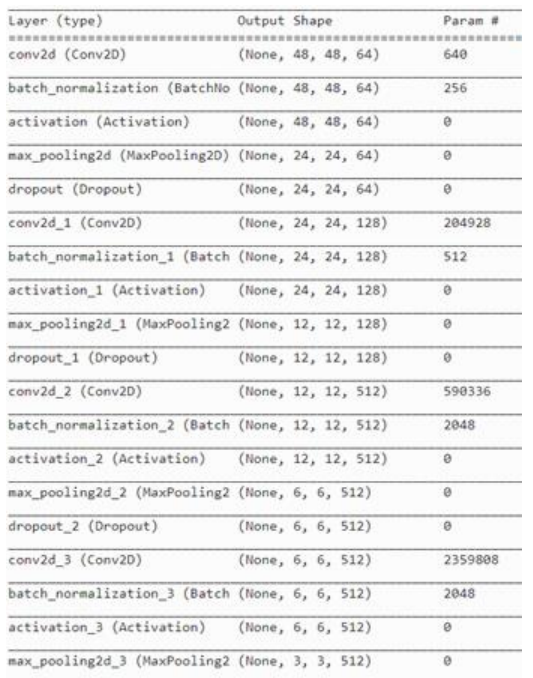
\includegraphics[width=0.5\textwidth, height=5cm]{anh1.png}
    \caption{depicts the analysis of the proposed FER model built using Keras
}
    \label{fig:anh1}
 
\end{figure}

\begin{figure}[h]
    \centering
    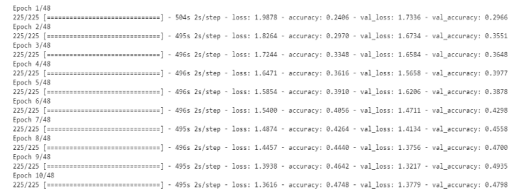
\includegraphics[width=0.5\textwidth, height=2cm]{anh2.png}
    \caption{depict the accuracy and loss of the value }
    \label{fig:anh2}
\end{figure}

\begin{figure}[h]
    \centering
    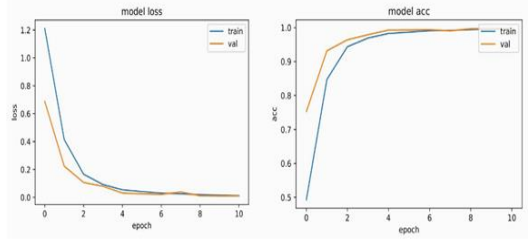
\includegraphics[width=0.5\textwidth, height=2cm]{anh3.png}
    \caption{depict the accuracy of training and validation (testing) data as well as model loss during the CNN training process. }
    \label{fig:anh3}
\end{figure}
After executing the OpenCV model the facial expressions and emotions are detected as given below figures 4, 5, 6 indicates the 3 major emotions.Those human facial expressions and emotions are happy emotion is recognized as depicted in the following figure 6, as well as the remaining emotions are identified as the depicted in the figure 4 and 5

\begin{figure}[h]
    \centering
    \begin{minipage}[b]{0.25\textwidth}
        \centering
        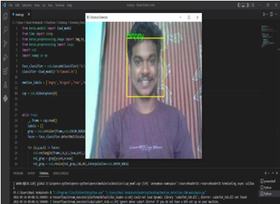
\includegraphics[width=0.5\textwidth, height=2.5cm]{happy.png}
        \caption{Happy emotions}
        \label{fig:happy}
    \end{minipage}
    \hspace{0.1\textwidth}
    \begin{minipage}[b]{0.25\textwidth}
        \centering
        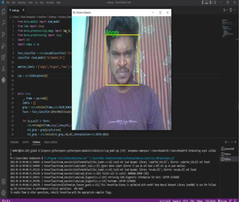
\includegraphics[width=0.5\textwidth, height=2.5cm]{angry.png}
        \caption{Angry emotions}
        \label{fig:angry}
    \end{minipage}
    \begin{minipage}[b]{0.25\textwidth}
        \centering
        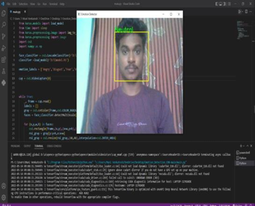
\includegraphics[width=0.5\textwidth, height=2.5cm]{neutral.png}
        \caption{Neutral emotions}
        \label{fig:neutral}
    \end{minipage}
\end{figure}

\section{Conclusion}
In this paper, we propose a two-layer convolutional neural network for extracting and classifying 7 human facial expressions from the FER Image dataset, comprising 35,887 images. The model achieves an 86.05\% accuracy, with both training and validation showing consistent performance. Future research aims to apply this approach to real-time applications using video sequences, facilitating feedback analysis and integration with electronic devices for enhanced control.



\begin{thebibliography}{00}
\bibitem{b1} J. L. Flores, A. E. G. Cutipa and R. L. Enciso, "Application of 
convolutional neural networks for static hand gestures recognition 
under different invariant features," 2017 IEEE XXIV International 
Conference on Electronics, Electrical Engineering and Computing 
(INTERCON), Cusco, 2017, pp. 1-4. 
\bibitem{b2} J. Shijie, W. Ping, J. Peiyi and H. Siping, "Research on data augmentation for image classification based on convolution neural networks," 2017 Chinese Automation Congress (CAC), Jinan, 2017, pp. 4165-4170. 
\bibitem{b3} A. Krizhevsky and G. Hinton. “Learning multiple layers of features from tiny images”, 2009. 
\bibitem{b4} Bouaziz, T Ramakrishnan, S. Raghavan, K. Grove, A.A.Omari, C 
Lakshminarayan, “ Character Recognition by Deep Learning: An 
Enterprise solution.”, IEEE Conference on Big Data, 2018. 
\bibitem{b5} P. Dhanalakshmi et al. (2022). Application of Machine Learning in Multi
Directional Model to Follow Solar Energy Using Photo Sensor 
Matrix. International journal of Photoenergy; 9:1-9.
\bibitem{b6} Li and W. Deng, “Deep facial expression recognition: A survey,” arXiv preprint arXiv:1804.08348, 2018.  
\end{thebibliography}

\end{document}
